% Detailed Research Plan -- Adaptive Task Allocation for Heterogeneous Bio-Inspired Agents
% Compiles on Overleaf with the default pdfLaTeX compiler. Single file, no .bib needed.

\documentclass[11pt,a4paper]{article}

\usepackage[T1]{fontenc}
\usepackage{newtxtext,newtxmath}
\usepackage[a4paper,margin=1in]{geometry}
\usepackage{microtype}
\usepackage{parskip}
\usepackage{booktabs,tabularx,array}
\usepackage{enumitem}
\usepackage{titlesec}
\usepackage[font=small,labelfont=bf,labelsep=period]{caption}
\usepackage{xcolor}
\usepackage{tikz}
\usetikzlibrary{positioning,arrows.meta,fit}
\usepackage{pgfgantt}
\usepackage{placeins}
\usepackage[hidelinks]{hyperref}

% ---- Details to fill in before submitting ---------------------------------
% Roll number of the junior member. Replace the rule with the number, e.g. 24/CS/123.
\newcommand{\juniorroll}{\rule{1.9cm}{0.4pt}}
% ---------------------------------------------------------------------------

\titleformat{\section}{\normalfont\large\bfseries}{\thesection}{0.7em}{}
\titleformat{\subsection}{\normalfont\normalsize\bfseries}{\thesubsection}{0.6em}{}
\titlespacing*{\section}{0pt}{16pt}{4pt}
\titlespacing*{\subsection}{0pt}{10pt}{2pt}
\setlist{itemsep=2pt,topsep=3pt,leftmargin=1.5em}
\renewcommand{\arraystretch}{1.18}
\newcolumntype{L}{>{\raggedright\arraybackslash}X}
\newcolumntype{P}[1]{>{\raggedright\arraybackslash}p{#1}}
\newcommand{\head}[1]{\textbf{#1}}
\newcommand{\runin}[1]{\textbf{#1}\quad}
\hyphenation{meta-heu-ris-tic pher-o-mone}
\emergencystretch=1.2em

\begin{document}

\begin{center}
  {\LARGE\bfseries Adaptive Task Allocation for\\[3pt]
  Heterogeneous Bio-Inspired Agents\par}
  \vspace{12pt}
  {\large Detailed Research Plan\par}
  \vspace{5pt}
  Final Year B.Tech Project, 2026--27\\
  Department of Computer Science and Engineering\\
  Delhi Technological University\par
  \vspace{8pt}
  {\small Submitted to Dr.~Yeshwant Singh, Group Faculty Coordinator (Group A4), on 12 October 2026}
\end{center}
\vspace{2pt}

\section{Group Details}

\begin{tabularx}{\textwidth}{@{}P{5.0cm}L@{}}
\toprule
\head{Project title} & Adaptive Task Allocation for Heterogeneous Bio-Inspired Agents \\
\head{Group ID} & A4 \quad (BTP Group No.\ GP105) \\
\head{Group Faculty Coordinator} & Dr.~Yeshwant Singh \\
\head{Guide} & Prof.~Shailender Kumar, Department of CSE \\
\head{Co-guide} & None \\
\bottomrule
\end{tabularx}

\vspace{6pt}

\begin{tabularx}{\textwidth}{@{}P{3.6cm}P{2.1cm}LP{2.3cm}@{}}
\toprule
\head{Name} & \head{Roll No.} & \head{Programme and year} & \head{Signature} \\
\midrule
Nikshay Yadav & 23/CS/284 & B.Tech CSE, final year & \\[7pt]
Madan Raj Murugesan & 23/CS/234 & B.Tech CSE, final year & \\[7pt]
Aryan Varshney & \juniorroll & B.Tech CSE, third year (junior member) & \\[7pt]
\bottomrule
\end{tabularx}

\vspace{14pt}
\hfill Signature of the guide:\enspace\rule{5cm}{0.4pt}

\section{Abstract and Problem Statement}

\subsection{Abstract}

Multi-agent systems built on large language models (LLMs) usually fix one way of working together before
the task is seen: a debate, a pipeline of roles, or a manager with workers. Real tasks are mixed. One part
needs a search over many candidate paths, another needs several independent opinions to be reconciled, and a
third is routine work that one worker can finish alone. When the same coordination pattern is applied to all
of them, the system pays for messages and tokens that do not improve the answer, and recent studies report
that such systems often fail to beat a well-prompted single agent. This project asks whether a coordinator
that picks a different coordination mechanism for each subtask can do better within the same budget. The
mechanisms are taken from animal behavior and written as ordinary algorithms: reinforced search (ant),
evidence accumulation with cross inhibition (bee), bounded local execution (octopus), tool-prerequisite
planning (crow) and checkpoint-based recovery (starfish), with two more kept as extensions. We will build
the framework, profile each mechanism on planning, tool-use and reasoning tasks whose answers can be checked
automatically, and learn a lightweight selector from the recorded outcomes. Adaptive allocation will be
compared with a single agent, the best single mechanism, fixed and random allocation, and a conventional
coordinator with specialist agents that is given the same model, tools and budget. The result will be a
working prototype and a measured account of when a mix of mechanisms helps and when it does not.

\subsection{Problem statement}

An LLM multi-agent system splits a task among agents that exchange messages. The split is useful only if
the way the agents coordinate suits the work. A subtask with many possible solution paths benefits from
exploration that remembers what worked. A subtask with a few competing answers needs those answers to be
compared and one of them chosen. A well-specified subtask needs no discussion at all, and involving the
coordinator at every step only adds cost. Current systems mostly choose one pattern for the whole task. The
evidence reviewed in Section~\ref{sec:lit} shows the consequence: the same architecture that improves one
kind of task by a large margin makes another kind worse~\cite{kim2025scaling}, and many failures can
be traced to system design and coordination and not only to the underlying model~\cite{cemri2025mast}.

We state the problem as follows. A task is decomposed into a dependency graph $G=(V,E)$ of subtasks. A pool
$\mathcal{M}=\{m_1,\dots,m_K\}$ of coordination mechanisms is available behind one interface, together with
a direct route that answers a subtask with a single model call. For each subtask $v$ that becomes ready, the
coordinator chooses $\pi(v)\in\mathcal{M}\cup\{\text{direct}\}$ from features it can observe before
execution and from the outcomes it has recorded so far. The aim is to maximize the probability that the
final answer is correct while the total cost, counted in tokens and model calls and including the
coordinator's own share, stays within a budget $B$. A wrong choice is paid for twice, once in wasted budget
and once in the reallocation that follows, so routing errors and communication overhead are part of the
problem and not side effects.

Three things are unknown and are what the project sets out to measure. It is not known whether mechanisms
that share one backbone model really differ in what they are good at. If they do, it is not known whether a
selector can exploit the difference using cheap features. And it is not known whether the biological
mechanisms add anything over well-designed conventional agents once compute is held equal.

\subsection{Objectives and research questions}

\begin{enumerate}[label=O\arabic*.]
  \item Build a modular coordinator with a common interface for heterogeneous mechanisms, starting with ant,
        bee and octopus and designed to take all seven proposed modules.
  \item Measure the strengths of each mechanism across task families and build capability profiles from
        correctness, cost and latency.
  \item Design allocation policies, first rule-based and then learned from recorded outcomes, and test
        them within a fixed budget.
  \item Separate the effect of the mechanisms from the effect of extra computation, using matched
        baselines and component ablations.
  \item Test recovery from injected failures and find the point at which coordination stops paying for
        itself.
\end{enumerate}

The objectives correspond to the five research questions of the approved synopsis. \textbf{RQ1:} Do the
mechanisms have complementary strengths? \textbf{RQ2:} Can dynamic allocation improve performance within a
fixed budget? \textbf{RQ3:} What value do the biological mechanisms add? \textbf{RQ4:} Can the framework
adapt to failures and changing task requirements? \textbf{RQ5:} When does coordination become inefficient?

\section{Brief Literature Review}
\label{sec:lit}

\runin{Fixed workflows and their cost.}
Most LLM multi-agent frameworks fix the roles and the communication pattern when the system is designed.
He, Treude and Lo~\cite{he2025lma} review 71 primary studies of such systems in software engineering and
place the optimization of agent collaboration as the second phase of their research agenda, after the
capabilities of individual agents. The cost of fixed designs is now documented. Cemri et
al.~\cite{cemri2025mast} annotated more than 1,600 execution traces from seven popular frameworks and
derived a taxonomy of 14 failure modes in three groups: system design, inter-agent misalignment and task
verification. Wang et al.~\cite{wang2024rethinking} found that a single agent with a strong prompt comes
close to the best multi-agent discussion method on a range of reasoning benchmarks. Zhang et
al.~\cite{zhang2025agentprune} treated redundant communication as a problem in its own right and showed that
many messages can be pruned. The most systematic evidence is from Kim et al.~\cite{kim2025scaling}, who
compared a single agent with four multi-agent architectures on six benchmarks and three model families
under standardized tools, prompts and compute. Relative to the single agent, performance changed by between
$+80.8\%$ on a decomposable financial reasoning task and $-70.0\%$ on sequential planning. Their conclusion,
that coordination helps only when it matches the structure of the task, is the starting point of this
project.

\runin{Adaptive topology and routing.}
A second line of work lets the structure depend on the task. GPTSwarm~\cite{zhuge2024gptswarm} describes
agents as computational graphs and optimizes both the prompts at the nodes and the connections between
them. DyLAN~\cite{liu2024dylan} selects a team for a task using an agent importance score.
G-Designer~\cite{zhang2025gdesigner} generates a communication topology for each task with a variational
graph auto-encoder, and AFlow~\cite{zhang2025aflow} searches over workflows written as code using Monte
Carlo tree search. RouteLLM~\cite{ong2025routellm} learns to send each query to a stronger or a weaker
model. MasRouter~\cite{yue2025masrouter} brings these decisions together: a cascaded controller chooses the
collaboration mode, the agent roles and the LLM for each role, and reports up to 52\% lower overhead than
earlier methods on HumanEval. Work from 2026 moves in the same direction.
GraphPlanner~\cite{feng2026graphplanner} generates a routing workflow for each query as a Markov decision
process, AdaptOrch~\cite{yu2026adaptorch} picks one of four topologies from the dependency graph of the
task, and Symphony-Coord~\cite{guan2026symphony} treats agent selection as an online bandit problem. These
systems establish that the right structure depends on the task. What they select among are roles, models
and graph shapes, in most cases once per query.

\runin{Bio-inspired coordination with LLMs.}
Wu et al.~\cite{wu2025ecllm} survey the two-way relationship between LLMs and evolutionary computation,
including LLMs that generate and improve optimization algorithms. Two recent systems apply swarm ideas to
agent coordination directly. AMRO-S~\cite{wang2026amros} models routing as path selection over a pool of
agents and applies ant colony optimization, with separate pheromone memories for different task types and a
small fine-tuned model that infers the intent of a query. SwarmSys~\cite{li2025swarmsys} cycles explorer,
worker and validator agents and uses a pheromone-inspired reinforcement rule for task allocation. Both are
preprints and both rely on a single, ant-like metaphor. There is also a skeptical reading. Rahman et
al.~\cite{rahman2026swarms} re-implemented Boids and ant colony optimization with LLM agents and found that
the LLM version of Boids needed about 300 times the computation time of the classical one. Outside the LLM
setting, Dama\v{s}evi\v{c}ius and Maskeli\={u}nas~\cite{damasevicius2021} combine the bat and krill herd
algorithms by switching agents between them according to performance, which is an early form of the
selection studied here. Camacho-Villal\'on et al.~\cite{camacho2023} analyzed six highly cited animal-named
optimizers component by component and argued that their metaphors hide ideas that already existed under
other names. We take this as a design rule: every module in this project is specified by what it computes,
and each one is tested against a plain counterpart that lacks its distinguishing component.

\runin{Biological basis and software counterparts.}
Seeley et al.~\cite{seeley2012} showed that scout bees committed to one nest site deliver stop signals to
scouts advertising a rival site, and that this cross inhibition lets a swarm settle on one option even when
two are equally good. Its nearest software relative is majority voting over independent
samples~\cite{wang2023selfconsistency}, which has no inhibition and no quorum. Sumbre et
al.~\cite{sumbre2001} showed that the arm extension of the octopus is produced by a motor program in the
arm itself, with the brain issuing the command but not the details, a division that resembles a coordinator
handing a bounded job to a worker. Taylor et al.~\cite{taylor2007} observed New Caledonian crows using a
short tool to obtain a longer one that could reach food. In LLM systems the corresponding ideas are tool
making and reuse~\cite{cai2024latm}, planning of function calls as a dependency graph~\cite{kim2024llmcompiler},
and tool learning more generally~\cite{qin2025tool}. Kano et al.~\cite{kano2017} built a brittle-star-like
robot that adapts immediately to the loss of arms through decentralized control. For LLM agents, Huang et
al.~\cite{huang2025resilience} injected faulty agents into six systems and found that hierarchical
structures lost the least performance (5.5\%), while Zhang et al.~\cite{zhang2025whowhen} showed that even
the best automatic method names the agent responsible for a failure only 53.5\% of the time. Two further
sources inform the coordinator. Theraulaz et al.~\cite{theraulaz1998} modeled division of labor in insect
colonies by letting each completed task lower an individual's response threshold for that task, so that
specialists emerge without central assignment. Experience stores for LLM agents~\cite{zhao2024expel,zhang2025memory}
provide the software form of the same idea and of the proposed elephant module.

\runin{Gap.}
Table~\ref{tab:related} places the project next to the closest systems. To our knowledge, no study has put
several coordination mechanisms with different control flow, memory and stopping rules behind one interface
and measured, at equal budget, which of them suits which kind of subtask. The bio-inspired systems that
exist use one mechanism and do not separate its contribution from that of the extra computation it spends.
Recovery from failure is studied apart from routing, although a reallocation is a routing decision. The
project addresses these three points with one framework and one evaluation protocol.

\begin{table}[h]
\centering\small
\caption{Closest prior systems and the position of this project.}
\label{tab:related}
\begin{tabularx}{\textwidth}{@{}P{3.5cm}P{4.4cm}LP{2.0cm}@{}}
\toprule
\head{System} & \head{What is adapted} & \head{How} & \head{Bio-inspired} \\
\midrule
GPTSwarm~\cite{zhuge2024gptswarm} & Node prompts and graph edges & Graph optimizers & No \\
G-Designer~\cite{zhang2025gdesigner} & Communication topology & Graph auto-encoder & No \\
AFlow~\cite{zhang2025aflow} & Whole workflow, as code & Monte Carlo tree search & No \\
MasRouter~\cite{yue2025masrouter} & Collaboration mode, roles, LLMs & Cascaded controller network & No \\
AdaptOrch~\cite{yu2026adaptorch} & One of four topologies & Task dependency graph & No \\
Symphony-Coord~\cite{guan2026symphony} & Agent chosen for a task & Online bandit & No \\
AMRO-S~\cite{wang2026amros} & Path through the agent pool & Ant colony optimization & Ant \\
SwarmSys~\cite{li2025swarmsys} & Agent--task matching & Pheromone-style reinforcement & Swarm \\
\midrule
This project & Coordination mechanism for each subtask & Rules, then a selector learned from outcomes &
Several, each with an ablation \\
\bottomrule
\end{tabularx}
\end{table}

\subsection{Five primary references}

The notice asks for five references from reputed venues published within the last five years. They are
references \cite{yue2025masrouter}--\cite{wu2025ecllm} in the list at the end and are summarized in
Table~\ref{tab:primary}. The remaining references support specific statements in this plan; the older
biological papers among them are cited as sources of the mechanisms and not as recent related work.

\begin{table}[h]
\centering\small
\caption{Primary references and their use in the project.}
\label{tab:primary}
\begin{tabularx}{\textwidth}{@{}P{0.8cm}P{4.6cm}L@{}}
\toprule
\head{Ref.} & \head{Venue and year} & \head{Use in this project} \\
\midrule
\cite{yue2025masrouter} & ACL, 2025 & Formulation of routing in multi-agent systems; the closest related
method, whose benchmarks we reuse for the reasoning tasks. \\
\cite{zhuge2024gptswarm} & ICML, 2024 & View of an agent system as a graph whose connections can be
optimized. \\
\cite{cemri2025mast} & NeurIPS, 2025 & Failure taxonomy, used to label a sample of our failed runs. \\
\cite{he2025lma} & ACM Trans.\ Softw.\ Eng.\ Methodol., 2025 & Review of role-based multi-agent systems;
basis for the conventional specialist baseline. \\
\cite{wu2025ecllm} & IEEE Trans.\ Evol.\ Comput., 2025 & Survey connecting LLMs with evolutionary and swarm
computation. \\
\bottomrule
\end{tabularx}
\end{table}

\section{Proposed Methodology}

\subsection{Architecture}

Figure~\ref{fig:arch} shows the planned system. The coordinator decomposes the incoming task into a
dependency graph, selects a mechanism for each subtask that is ready, dispatches it with a share of the
budget, verifies the result and reallocates the subtask if verification fails. Every module implements the
same call, which takes a subtask, its context and a budget, and returns the output, a confidence estimate,
the cost (prompt and completion tokens, model calls and elapsed time), a status flag and the full trace.
All modules use the same backbone model and the same tools through one client. They differ only in control
flow, communication rules, memory updates and stopping conditions, so a difference in results can be
attributed to the mechanism.

\begin{figure}[h]
\centering
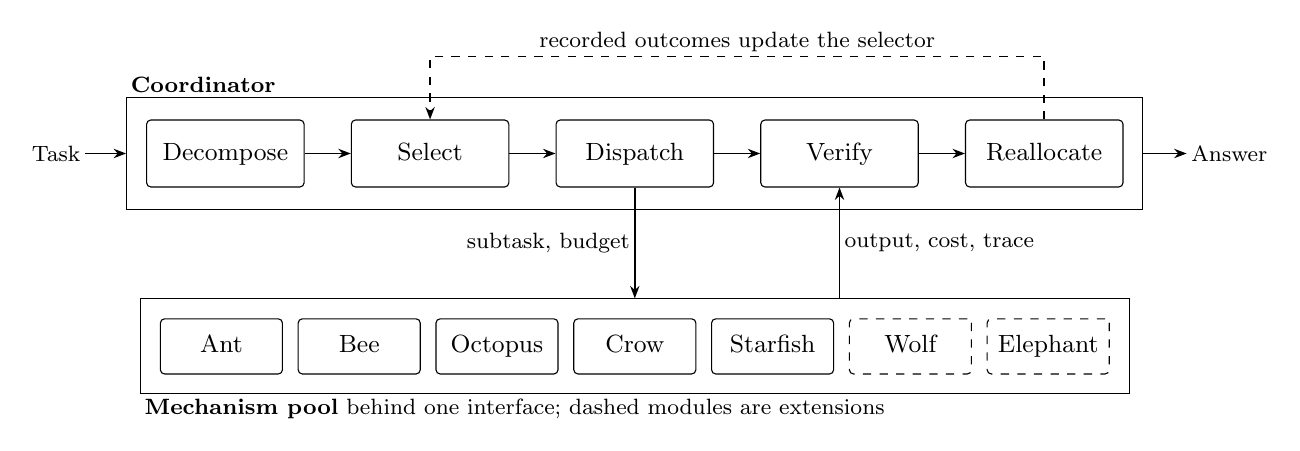
\begin{tikzpicture}[font=\small,
  box/.style={draw, rounded corners=1.5pt, minimum height=8.5mm, minimum width=20mm, align=center,
              inner sep=3pt, text height=1.6ex, text depth=0.5ex},
  mod/.style={draw, rounded corners=1.5pt, minimum height=7mm, minimum width=15.5mm, align=center,
              inner sep=2pt, text height=1.6ex, text depth=0.5ex},
  arr/.style={-{Stealth[length=4.5pt]}, semithick},
  lab/.style={font=\footnotesize, inner sep=1.5pt}]
  % coordinator stages
  \node[box] (dec) at (0,0) {Decompose};
  \node[box] (sel) at (2.6,0) {Select};
  \node[box] (dis) at (5.2,0) {Dispatch};
  \node[box] (ver) at (7.8,0) {Verify};
  \node[box] (rea) at (10.4,0) {Reallocate};
  \draw[arr] (dec) -- (sel);
  \draw[arr] (sel) -- (dis);
  \draw[arr] (dis) -- (ver);
  \draw[arr] (ver) -- (rea);
  \node[draw, fit=(dec)(rea), inner xsep=7pt, inner ysep=8pt] (coord) {};
  \node[lab, anchor=south west] at (coord.north west) {\textbf{Coordinator}};
  % task in, answer out
  \node[lab] (task) at (-2.15,0) {Task};
  \draw[arr] (task) -- (coord.west);
  \node[lab] (ans) at (12.75,0) {Answer};
  \draw[arr] (coord.east) -- (ans);
  % mechanism pool
  \node[mod] (ant) at (-0.05,-2.45) {Ant};
  \node[mod] (bee) at (1.70,-2.45) {Bee};
  \node[mod] (oct) at (3.45,-2.45) {Octopus};
  \node[mod] (cro) at (5.20,-2.45) {Crow};
  \node[mod] (sta) at (6.95,-2.45) {Starfish};
  \node[mod, dashed] (wol) at (8.70,-2.45) {Wolf};
  \node[mod, dashed] (ele) at (10.45,-2.45) {Elephant};
  \node[draw, fit=(ant)(ele), inner xsep=7pt, inner ysep=7pt] (pool) {};
  \node[lab, anchor=north west] at (pool.south west) {\textbf{Mechanism pool} behind one interface; dashed modules are extensions};
  % flows
  \draw[arr] (dis.south) -- node[lab, left, pos=0.5] {subtask, budget} (dis.south |- pool.north);
  \draw[arr] (ver.south |- pool.north) -- node[lab, right, pos=0.5] {output, cost, trace} (ver.south);
  \draw[arr, dashed] (rea.north) -- ++(0,0.8) -| node[lab, above, pos=0.25] {recorded outcomes update the selector} (sel.north);
\end{tikzpicture}
\caption{Planned architecture. The coordinator runs the five stages for every ready subtask and keeps the
task graph, the remaining budget, the execution status and the outcome log.}
\label{fig:arch}
\end{figure}

\subsection{Mechanisms}

Table~\ref{tab:mech} defines each module by its behavior. The last column gives the plain counterpart
against which it will be ablated. Ant, bee and octopus are built first. Crow and starfish follow in the
second semester. Wolf and elephant are exploratory and will be attempted only if the core study is on
schedule.

\begin{table}[h]
\centering\small
\caption{Mechanisms as computational behavior.}
\label{tab:mech}
\setlength{\tabcolsep}{4pt}
\begin{tabularx}{\textwidth}{@{}P{1.45cm}LP{3.0cm}P{2.9cm}P{3.1cm}@{}}
\toprule
\head{Module} & \head{Control flow} & \head{State kept} & \head{Stops when} & \head{Plain counterpart} \\
\midrule
Ant & Samples candidate solution paths in proportion to learned weights, executes and scores them &
Weights per task feature and step choice, reinforced on success and evaporated each round &
Best path is stable for several rounds, or budget is spent & Same sampler with uniform, fixed weights \\
Bee & Several scouts answer independently; supporters of an option recruit others and inhibit rivals &
Support for each option, within one subtask & One option reaches a quorum, or budget is spent &
Majority vote over the same number of samples \\
Octopus & Receives a goal and a budget, runs its own act--observe loop, returns a summary &
Private scratchpad, dropped after the report & Goal check passes, or local budget is spent &
Worker that reports to the coordinator after every step \\
Crow & Works back from the goal to the tool outputs it depends on; may write and cache a helper tool &
Prerequisite graph and cached helper tools & All prerequisites are met and the final call is verified &
Step-by-step tool use without a plan \\
Starfish & Wraps another module; checkpoints its state and reassigns the remaining work after a failure &
Checkpoints & Subtask completes, or retries are exhausted & Restart of the whole subtask \\
Wolf & Parallel explorers with a penalty on overlapping search & Shared record of covered ground &
Coverage target or budget & Independent parallel explorers \\
Elephant & Retrieves similar past episodes and their outcomes before acting & Episode store across tasks &
After one retrieval-augmented attempt & Same attempt without retrieval \\
\bottomrule
\end{tabularx}
\end{table}

Two of the update rules are given here because the ablations refer to them. In the ant module a choice $c$
made under task feature $f$ has weight $\tau_{f,c}$. Choices are sampled with probability proportional to
$\tau_{f,c}^{\alpha}\,\eta_{f,c}^{\beta}$, where $\eta_{f,c}$ is the model's own prior for the choice, and
after a verified reward $r\in[0,1]$ the weight is updated as
\[
  \tau_{f,c}\;\leftarrow\;(1-\rho)\,\tau_{f,c}+\rho\,r ,
\]
with evaporation rate $\rho$. In the bee module $x_i$ is the fraction of scouts committed to option $i$ and
$q_i$ is the quality of the evidence for it. A simplified form of the model in~\cite{seeley2012} is
\[
  x_i^{t+1}=x_i^{t}+\gamma\,q_i\,u^{t}-\sigma\,x_i^{t}\sum_{j\neq i}x_j^{t},
  \qquad u^{t}=1-\sum_{j}x_j^{t},
\]
and the module answers with option $i$ as soon as $x_i\geq\theta$. Setting $\rho=0$ or $\sigma=0$ gives the
plain counterparts in Table~\ref{tab:mech}. All parameters will be tuned on development tasks only.

\subsection{Allocation policy}

The coordinator describes each ready subtask by features that are available before execution: the number
of candidate options, whether the result can be checked automatically, the tools it needs and the depth of
their dependencies, the number of sibling subtasks that are ready at the same time, an estimate of its
length, and the recorded outcomes of similar subtasks. Allocation is developed in two stages. The first is
a small rule table derived from the capability profiles of RQ1. The second is a contextual bandit over the
same features, starting with LinUCB~\cite{li2010linucb}, whose arms are the mechanisms and the direct
single-call route. Its reward for a subtask is $s-\lambda c$, where $s\in\{0,1\}$ is verified success, $c$
is the normalized token cost and $\lambda$ sets the trade-off. The selector is trained on development tasks
and frozen before the held-out evaluation. It reinforces the choices that worked, which is the same
principle as the threshold reinforcement in~\cite{theraulaz1998}, applied at the level of the coordinator.

\subsection{Evaluation plan}

\runin{Tasks.}
All tasks have answers that a program can check, so no LLM judge is needed. Three families are planned:
planning, using PlanBench-style instances~\cite{valmeekam2023planbench} and the validation split of
TravelPlanner~\cite{xie2024travelplanner}; tool use, using a subset of the GAIA validation
set~\cite{mialon2024gaia} and a small suite of our own built on deterministic local tools; and reasoning,
using arithmetic and multi-hop sets from the routing literature~\cite{yue2025masrouter} so that our numbers
can be read against published ones. In addition we will generate synthetic tasks in which the number of
alternatives, the dependency depth, the parallel width and the fault rate are set by us. These allow the
hypotheses of RQ1 to be tested one factor at a time. Each family is split into development and held-out
parts, and one task variant per family is withheld completely to test generalization.

\runin{Systems compared.}
(i) A single agent; (ii) each mechanism used alone, which also gives the best single mechanism in
hindsight; (iii) fixed allocation, with one mechanism assigned to each task family by hand; (iv) random
allocation; (v) a conventional coordinator with specialist agents (planner, researcher, executor, critic)
that has the same model, tools, memory access and budget; and (vi) adaptive allocation in its rule-based
and learned forms. Every system receives the same cap on tokens per task. Results will be reported at
several budget levels, as curves of success against cost, since a single operating point can favor any
method.

\runin{Measurements.}
Task success; tokens divided into coordinator, worker and inter-agent communication; model calls;
elapsed time; successes per million tokens; routing regret against the best mechanism in hindsight; and the
recovery rate after injected faults. For RQ4, worker timeouts, tool errors and corrupted intermediate
results will be injected at fixed rates, in the manner of~\cite{huang2025resilience}. A sample of failed
runs will be labeled with the failure taxonomy of~\cite{cemri2025mast}.

\runin{Ablations and analysis.}
Reinforcement and evaporation, inhibition, and local autonomy are removed one at a time, the selector is
replaced by a random one, and outcome memory is switched off. Each configuration is run at least three
times with different seeds. We will report bootstrap 95\% confidence intervals and paired tests on the same
task instances, and will state results that go against the hypothesis as plainly as those that support it.

\runin{Threats to validity.}
Hosted models change without notice, so model versions will be pinned, responses cached and the main
comparison repeated on an open-weight model with fixed weights. Public benchmarks may have been seen in
training, which is one reason for the synthetic and in-house tasks. Our sample sizes are limited by budget,
and the confidence intervals will show how much each claim can bear.

\section{Technical Requirements}

\begin{table}[h]
\centering\small
\begin{tabularx}{\textwidth}{@{}P{2.3cm}L@{}}
\toprule
\head{Hardware} &
Two personal laptops for development. The reference machine has an Intel Core i5-1240P, 16~GB RAM and an
NVIDIA RTX~2050 (4~GB) and runs Linux; this is enough for the orchestration code, the tool sandbox and
small local models for smoke tests. Free cloud notebooks (Kaggle, Google Colab) with a 16~GB T4-class GPU
for open-weight models. About 20~GB of storage for traces and response caches. No dedicated server or
departmental GPU is required. \\
\midrule
\head{Software} &
Python 3.11 or later with \texttt{asyncio}; Pydantic for message schemas; NetworkX for the task graph;
SQLite and JSON Lines for traces; NumPy and scikit-learn for the selector; pandas, SciPy and Matplotlib for
analysis; pytest for tests; Docker for sandboxed tool execution; Hugging Face Transformers and Datasets,
with Ollama or \texttt{llama.cpp} to serve open-weight models; Git and GitHub for version control
(\url{https://github.com/Nikshay1/BTP}); \LaTeX{} for the report. The orchestration layer will be written
by us instead of being taken from an agent framework, because every message has to be metered. \\
\midrule
\head{Models} &
One small hosted model as the primary backbone, reached through an API with a free or low-cost tier (for
example the Gemini API, Groq or OpenRouter), and one open-weight instruction-tuned model of 7--8 billion
parameters (Llama, Qwen or Mistral family) in 4-bit quantization as the second backbone. The exact models
will be fixed after the pilot and then kept unchanged. \\
\midrule
\head{Compute} &
No model training is involved; the cost is inference. Table~\ref{tab:compute} gives the planning estimate
of about 14,700 task runs. At 8,000 to 15,000 tokens per run this is roughly 120 to 220 million tokens,
most of them input tokens. Response caching, development on small subsets and free tiers reduce the paid
share. At present prices for small hosted models the full budget is on the order of a few thousand rupees,
and the figure will be revised after the pilot in December. \\
\bottomrule
\end{tabularx}
\end{table}

\begin{table}[h]
\centering\small
\caption{Planning estimate of experiment size.}
\label{tab:compute}
\begin{tabular}{@{}llr@{}}
\toprule
\head{Stage} & \head{Systems $\times$ tasks $\times$ runs} & \head{Task runs} \\
\midrule
Capability profiling (RQ1) & $4 \times 300 \times 3$ & 3,600 \\
Main comparison (RQ2, RQ3) & $6 \times 300 \times 3$ & 5,400 \\
Ablations (RQ3) & $5 \times 300 \times 2$ & 3,000 \\
Fault injection (RQ4) & $3 \times 3\ \text{fault settings} \times 150 \times 2$ & 2,700 \\
\midrule
Total & & 14,700 \\
\bottomrule
\end{tabular}
\end{table}

\section{Expected Outcomes}

\begin{itemize}
  \item \textbf{A modular research prototype.} A coordinator with a common interface for heterogeneous
        bio-inspired agents, validated first with three mechanisms and able to take all seven.
  \item \textbf{Capability profiles.} Evidence of which mechanism suits which class of subtask, and of
        when combining them is useful.
  \item \textbf{Comparative results.} Task success, token use, inference cost, completion time and recovery
        after controlled failures, for the adaptive system and for every baseline at equal budget.
  \item \textbf{Component-level analysis.} Ablations that separate the effects of adaptive routing, memory,
        communication and the agent-specific mechanisms.
  \item \textbf{Reproducible materials.} Code, configurations, evaluation scripts and experiment logs in a
        public repository, supporting the final report and a possible conference submission.
\end{itemize}

The working hypothesis is that adaptive allocation improves task success at an equal budget, or lowers cost
at comparable success. We will count it as supported if, on held-out tasks, the adaptive system beats the
best single mechanism on one of these two measures with a confidence interval that excludes zero. If the
conventional specialist coordinator does equally well, the conclusion will be that the gain comes from
allocation and not from the biological mechanisms, and the report will say so. Cases in which a single
agent is the better choice will be reported as the answer to RQ5.

\section{Timeline and Work Plan}

The plan covers the seventh and eighth semesters, from October 2026 to May 2027. Each column of
Figure~\ref{fig:gantt} is half a month. Evaluation dates are indicative and will follow the department
schedule.

\begin{figure}[h]
\centering
\begin{ganttchart}[
    x unit=0.545cm,
    y unit chart=0.54cm,
    y unit title=0.52cm,
    canvas/.style={draw=black!45, line width=0.4pt},
    hgrid={*1{draw=black!13}},
    vgrid={*1{draw=black!9}},
    title/.style={draw=black!45, line width=0.4pt, fill=none},
    title label font=\footnotesize,
    title height=1,
    bar/.style={draw=none, fill=black!62},
    bar height=0.46,
    bar top shift=0.27,
    bar label font=\footnotesize,
    milestone/.style={draw=black, fill=black, shape=diamond, inner sep=1.6pt},
    milestone label font=\footnotesize\itshape,
    milestone height=0.46,
    milestone top shift=0.27,
    milestone left shift=-0.1,
    milestone right shift=-0.9,
    inline=false
  ]{1}{16}
  \gantttitle{2026}{6}\gantttitle{2027}{10}\\
  \gantttitle{Oct}{2}\gantttitle{Nov}{2}\gantttitle{Dec}{2}\gantttitle{Jan}{2}%
  \gantttitle{Feb}{2}\gantttitle{Mar}{2}\gantttitle{Apr}{2}\gantttitle{May}{2}\\
  \ganttbar{Literature study, research plan}{1}{3}\\
  \ganttbar{Framework core and logging}{2}{4}\\
  \ganttbar{Ant, bee, octopus modules}{3}{5}\\
  \ganttbar{Task suites and baselines}{3}{6}\\
  \ganttbar{Pilot, capability profiles (RQ1)}{5}{8}\\
  \ganttbar{Allocation policies (RQ2)}{7}{10}\\
  \ganttbar{Specialist baseline, ablations (RQ3)}{9}{11}\\
  \ganttbar{Crow, starfish; fault study (RQ4)}{9}{12}\\
  \ganttbar{Overhead and budget study (RQ5)}{11}{12}\\
  \ganttbar[bar/.append style={fill=black!26}]{Wolf, elephant (if on schedule)}{11}{13}\\
  \ganttbar{Held-out evaluation, statistics}{12}{14}\\
  \ganttbar{Report, paper draft, code release}{13}{16}\\
  \ganttmilestone{Milestones M1--M5}{3}
  \ganttmilestone{}{6}
  \ganttmilestone{}{10}
  \ganttmilestone{}{14}
  \ganttmilestone{}{16}
\end{ganttchart}
\caption{Work plan, October 2026 to May 2027. The lighter bar is optional work.}
\label{fig:gantt}
\end{figure}

\begin{table}[h]
\centering\small
\caption{Milestones and deliverables.}
\label{tab:milestones}
\begin{tabularx}{\textwidth}{@{}P{0.9cm}P{3.1cm}L@{}}
\toprule
\head{No.} & \head{When} & \head{Deliverable} \\
\midrule
M1 & Mid-November 2026 & Coordinator, common interface and logging working end to end with one mechanism
on a toy task. \\
M2 & December 2026 & Ant, bee and octopus modules, task suites and baselines; pilot results for the
seventh-semester evaluation. \\
M3 & End of February 2027 & Capability profiles (RQ1) and both allocation policies evaluated on development
tasks (RQ2). \\
M4 & End of April 2027 & Held-out results, ablations (RQ3), fault study (RQ4) and overhead study (RQ5)
complete. \\
M5 & May 2027 & Final report, public code and logs, and a paper draft for the final evaluation. \\
\bottomrule
\end{tabularx}
\end{table}

\begin{table}[h]
\centering\small
\caption{Main risks and how the plan handles them.}
\label{tab:risks}
\begin{tabularx}{\textwidth}{@{}P{5.2cm}L@{}}
\toprule
\head{Risk} & \head{Response} \\
\midrule
API limits or cost exceed the estimate & Cache every response, develop on small subsets, use small models,
and fall back to open-weight models on free GPUs. \\
Results vary between runs or after a model update & Pinned model versions, fixed seeds, repeated runs and a
replication on an open-weight model. \\
The mechanisms do not differ in strengths & This is an answer to RQ1. The study then concentrates on cost
and overhead (RQ5) and the selector is reduced to choosing between direct and coordinated execution. \\
Seven modules are too many for two semesters & Work is staged: three core modules first, crow and starfish
next, wolf and elephant only if the core study is on schedule. \\
Full benchmarks are too long to run & Fixed subsets are chosen and recorded before any experiment is run. \\
\bottomrule
\end{tabularx}
\end{table}

The seventh semester is for building. By its end the coordinator, the three core modules, the task suites
and the baselines should run end to end, and the pilot should tell us what a task run costs and whether the
mechanisms differ at all. The eighth semester is for the study itself. Allocation policies come first,
since every later experiment depends on them. The matched baseline with its ablations, the fault study and
the overhead study share one harness and can run side by side. The last six weeks are kept for the held-out
evaluation and for writing. The bars that cross the end-semester examinations are deliberately long, since
little project work will be done in those weeks. Table~\ref{tab:milestones} lists the milestones and
Table~\ref{tab:risks} the main risks.

\FloatBarrier

\begingroup
\footnotesize
\setlength{\parskip}{0pt}
\begin{thebibliography}{99}
\setlength{\itemsep}{2pt}
\sloppy

\bibitem{yue2025masrouter}
Y.~Yue, G.~Zhang, B.~Liu, G.~Wan, K.~Wang, D.~Cheng, and Y.~Qi, ``MasRouter: Learning to route LLMs for
multi-agent systems,'' in \emph{Proc.\ 63rd Annu.\ Meeting Assoc.\ Comput.\ Linguistics (ACL)}, 2025,
pp.~15549--15572.

\bibitem{zhuge2024gptswarm}
M.~Zhuge, W.~Wang, L.~Kirsch, F.~Faccio, D.~Khizbullin, and J.~Schmidhuber, ``GPTSwarm: Language agents as
optimizable graphs,'' in \emph{Proc.\ 41st Int.\ Conf.\ Mach.\ Learn.\ (ICML)}, PMLR vol.~235, 2024,
pp.~62743--62767.

\bibitem{cemri2025mast}
M.~Cemri \emph{et al.}, ``Why do multi-agent LLM systems fail?,'' in \emph{Adv.\ Neural Inf.\ Process.\
Syst.\ (NeurIPS), Datasets and Benchmarks Track}, 2025.

\bibitem{he2025lma}
J.~He, C.~Treude, and D.~Lo, ``LLM-based multi-agent systems for software engineering: Literature review,
vision, and the road ahead,'' \emph{ACM Trans.\ Softw.\ Eng.\ Methodol.}, vol.~34, no.~5, pp.~1--30, 2025,
\href{https://doi.org/10.1145/3712003}{doi:~10.1145/3712003}.

\bibitem{wu2025ecllm}
X.~Wu, S.-H.~Wu, J.~Wu, L.~Feng, and K.~C.~Tan, ``Evolutionary computation in the era of large language
model: Survey and roadmap,'' \emph{IEEE Trans.\ Evol.\ Comput.}, vol.~29, no.~2, pp.~534--554, 2025,
\href{https://doi.org/10.1109/TEVC.2024.3506731}{doi:~10.1109/TEVC.2024.3506731}.

\bibitem{kim2025scaling}
Y.~Kim \emph{et al.}, ``Towards a science of scaling agent systems,''
\href{https://arxiv.org/abs/2512.08296}{arXiv:2512.08296}, 2025.

\bibitem{wang2024rethinking}
Q.~Wang, Z.~Wang, Y.~Su, H.~Tong, and Y.~Song, ``Rethinking the bounds of LLM reasoning: Are multi-agent
discussions the key?,'' in \emph{Proc.\ 62nd Annu.\ Meeting Assoc.\ Comput.\ Linguistics (ACL)}, 2024,
pp.~6106--6131.

\bibitem{zhang2025agentprune}
G.~Zhang \emph{et al.}, ``Cut the crap: An economical communication pipeline for LLM-based multi-agent
systems,'' in \emph{Proc.\ Int.\ Conf.\ Learn.\ Represent.\ (ICLR)}, 2025.

\bibitem{liu2024dylan}
Z.~Liu, Y.~Zhang, P.~Li, Y.~Liu, and D.~Yang, ``A dynamic LLM-powered agent network for task-oriented agent
collaboration,'' in \emph{Proc.\ 1st Conf.\ Lang.\ Model.\ (COLM)}, 2024.

\bibitem{zhang2025gdesigner}
G.~Zhang \emph{et al.}, ``G-Designer: Architecting multi-agent communication topologies via graph neural
networks,'' in \emph{Proc.\ 42nd Int.\ Conf.\ Mach.\ Learn.\ (ICML)}, 2025.

\bibitem{zhang2025aflow}
J.~Zhang \emph{et al.}, ``AFlow: Automating agentic workflow generation,'' in \emph{Proc.\ Int.\ Conf.\
Learn.\ Represent.\ (ICLR)}, 2025.

\bibitem{ong2025routellm}
I.~Ong \emph{et al.}, ``RouteLLM: Learning to route LLMs with preference data,'' in \emph{Proc.\ Int.\
Conf.\ Learn.\ Represent.\ (ICLR)}, 2025.

\bibitem{feng2026graphplanner}
T.~Feng, H.~Zhang, Z.~Lei, P.~Han, and J.~You, ``GraphPlanner: Graph memory-augmented agentic routing for
multi-agent LLMs,'' in \emph{Proc.\ Int.\ Conf.\ Learn.\ Represent.\ (ICLR)}, 2026.

\bibitem{yu2026adaptorch}
G.~Yu, ``AdaptOrch: Task-adaptive multi-agent orchestration in the era of LLM performance convergence,''
\href{https://arxiv.org/abs/2602.16873}{arXiv:2602.16873}, 2026.

\bibitem{guan2026symphony}
Z.~Guan \emph{et al.}, ``Symphony-Coord: Adaptive routing for multi-agent LLM systems,''
\href{https://arxiv.org/abs/2602.00966}{arXiv:2602.00966}, 2026.

\bibitem{wang2026amros}
X.~Wang \emph{et al.}, ``Efficient and interpretable multi-agent LLM routing via ant colony optimization,''
\href{https://arxiv.org/abs/2603.12933}{arXiv:2603.12933}, 2026.

\bibitem{li2025swarmsys}
R.~Li \emph{et al.}, ``SwarmSys: Decentralized swarm-inspired agents for scalable and adaptive reasoning,''
\href{https://arxiv.org/abs/2510.10047}{arXiv:2510.10047}, 2025.

\bibitem{rahman2026swarms}
M.~A.~U.~Rahman, M.~Schranz, and S.~Hayat, ``LLM-powered swarms: A new frontier or a conceptual stretch?,''
\emph{IEEE Intell.\ Syst.}, early access, 2026,
\href{https://doi.org/10.1109/MIS.2026.3728883}{doi:~10.1109/MIS.2026.3728883}.

\bibitem{damasevicius2021}
R.~Dama\v{s}evi\v{c}ius and R.~Maskeli\={u}nas, ``Agent state flipping based hybridization of heuristic
optimization algorithms: A case of bat algorithm and krill herd hybrid algorithm,'' \emph{Algorithms},
vol.~14, no.~12, art.~358, 2021.

\bibitem{camacho2023}
C.~L.~Camacho-Villal\'on, M.~Dorigo, and T.~St\"utzle, ``Exposing the grey wolf, moth-flame, whale,
firefly, bat, and antlion algorithms: Six misleading optimization techniques inspired by bestial
metaphors,'' \emph{Int.\ Trans.\ Oper.\ Res.}, vol.~30, no.~6, pp.~2945--2971, 2023.

\bibitem{seeley2012}
T.~D.~Seeley, P.~K.~Visscher, T.~Schlegel, P.~M.~Hogan, N.~R.~Franks, and J.~A.~R.~Marshall, ``Stop signals
provide cross inhibition in collective decision-making by honeybee swarms,'' \emph{Science}, vol.~335,
no.~6064, pp.~108--111, 2012.

\bibitem{wang2023selfconsistency}
X.~Wang \emph{et al.}, ``Self-consistency improves chain of thought reasoning in language models,'' in
\emph{Proc.\ Int.\ Conf.\ Learn.\ Represent.\ (ICLR)}, 2023.

\bibitem{sumbre2001}
G.~Sumbre, Y.~Gutfreund, G.~Fiorito, T.~Flash, and B.~Hochner, ``Control of octopus arm extension by a
peripheral motor program,'' \emph{Science}, vol.~293, no.~5536, pp.~1845--1848, 2001.

\bibitem{taylor2007}
A.~H.~Taylor, G.~R.~Hunt, J.~C.~Holzhaider, and R.~D.~Gray, ``Spontaneous metatool use by New Caledonian
crows,'' \emph{Curr.\ Biol.}, vol.~17, no.~17, pp.~1504--1507, 2007.

\bibitem{cai2024latm}
T.~Cai, X.~Wang, T.~Ma, X.~Chen, and D.~Zhou, ``Large language models as tool makers,'' in \emph{Proc.\
Int.\ Conf.\ Learn.\ Represent.\ (ICLR)}, 2024.

\bibitem{kim2024llmcompiler}
S.~Kim \emph{et al.}, ``An LLM compiler for parallel function calling,'' in \emph{Proc.\ 41st Int.\ Conf.\
Mach.\ Learn.\ (ICML)}, 2024.

\bibitem{qin2025tool}
Y.~Qin \emph{et al.}, ``Tool learning with foundation models,'' \emph{ACM Comput.\ Surv.}, vol.~57, no.~4,
pp.~1--40, 2025, \href{https://doi.org/10.1145/3704435}{doi:~10.1145/3704435}.

\bibitem{kano2017}
T.~Kano, E.~Sato, T.~Ono, H.~Aonuma, Y.~Matsuzaka, and A.~Ishiguro, ``A brittle star-like robot capable of
immediately adapting to unexpected physical damage,'' \emph{R.\ Soc.\ Open Sci.}, vol.~4, no.~12,
art.~171200, 2017.

\bibitem{huang2025resilience}
J.-T.~Huang \emph{et al.}, ``On the resilience of LLM-based multi-agent collaboration with faulty agents,''
in \emph{Proc.\ 42nd Int.\ Conf.\ Mach.\ Learn.\ (ICML)}, 2025.

\bibitem{zhang2025whowhen}
S.~Zhang \emph{et al.}, ``Which agent causes task failures and when? On automated failure attribution of
LLM multi-agent systems,'' in \emph{Proc.\ 42nd Int.\ Conf.\ Mach.\ Learn.\ (ICML)}, 2025.

\bibitem{theraulaz1998}
G.~Theraulaz, E.~Bonabeau, and J.-L.~Deneubourg, ``Response threshold reinforcements and division of labour
in insect societies,'' \emph{Proc.\ R.\ Soc.\ Lond.\ B}, vol.~265, no.~1393, pp.~327--332, 1998.

\bibitem{zhao2024expel}
A.~Zhao, D.~Huang, Q.~Xu, M.~Lin, Y.-J.~Liu, and G.~Huang, ``ExpeL: LLM agents are experiential learners,''
in \emph{Proc.\ AAAI Conf.\ Artif.\ Intell.}, vol.~38, no.~17, 2024, pp.~19632--19642.

\bibitem{zhang2025memory}
Z.~Zhang \emph{et al.}, ``A survey on the memory mechanism of large language model-based agents,''
\emph{ACM Trans.\ Inf.\ Syst.}, vol.~43, no.~6, pp.~1--47, 2025,
\href{https://doi.org/10.1145/3748302}{doi:~10.1145/3748302}.

\bibitem{li2010linucb}
L.~Li, W.~Chu, J.~Langford, and R.~E.~Schapire, ``A contextual-bandit approach to personalized news article
recommendation,'' in \emph{Proc.\ 19th Int.\ Conf.\ World Wide Web (WWW)}, 2010, pp.~661--670.

\bibitem{valmeekam2023planbench}
K.~Valmeekam, M.~Marquez, A.~Olmo, S.~Sreedharan, and S.~Kambhampati, ``PlanBench: An extensible benchmark
for evaluating large language models on planning and reasoning about change,'' in \emph{Adv.\ Neural Inf.\
Process.\ Syst.\ (NeurIPS), Datasets and Benchmarks Track}, 2023.

\bibitem{xie2024travelplanner}
J.~Xie \emph{et al.}, ``TravelPlanner: A benchmark for real-world planning with language agents,'' in
\emph{Proc.\ 41st Int.\ Conf.\ Mach.\ Learn.\ (ICML)}, 2024.

\bibitem{mialon2024gaia}
G.~Mialon, C.~Fourrier, C.~Swift, T.~Wolf, Y.~LeCun, and T.~Scialom, ``GAIA: A benchmark for general AI
assistants,'' in \emph{Proc.\ Int.\ Conf.\ Learn.\ Represent.\ (ICLR)}, 2024.

\end{thebibliography}
\endgroup

\end{document}
